\chapter{深度生成建模}\label{ch:overview-dgm}

\epigraph{
    \textit{我无法创造的东西，我不明白。}}{理查德·P·费曼}









深度生成模型 (DGM) 是学习高维数据（例如图像、文本、音频）概率分布的神经网络，因此它们可以生成类似于数据集的新示例。我们将模型分布表示为 $p_{\bphi}$ 数据分布 $p_{\mathrm{data}}$。给定一个有限的数据集，我们拟合 $\bphi$ 通过最小化损失来衡量距离 $p_{\bphi}$ 来自 $p_{\mathrm{data}}$。训练后，生成相当于运行模型的采样程序来绘制 $\rvx \sim p_{\bphi}$ （密度 $p_{\bphi}(\rvx)$ 可能可以也可能不能直接计算，具体取决于模型类别）。模型质量是根据生成的样本及其汇总统计数据与 $p_{\mathrm{data}}$，以及特定于任务的或感知指标。本章构建了这些想法背后的数学和概念基础。我们将问题形式化为 \Cref{sec:formulation-dgm}，呈现代表性模型类 \Cref{sec:examples-dgm}，并总结了实用的分类法 \Cref{sec:taxonomy}.

\chapterlearning{
  \item 用简单的语言解释生成模型试图从数据集中学习什么以及对数据分布进行建模意味着什么；
  \item 了解自回归模型、VAE、能量模型、归一化流、GAN 和扩散模型背后的核心思想，并了解它们在学习和生成新样本的方式上有何不同；
}{
如果您已经熟悉现代生成模型背后的基本思想，您可以浏览本章并在以后将其用作快速参考。
}














\newpage
\section{什么是深度生成建模？}\label{sec:formulation-dgm}





DGM 将来自未知且复杂的分布的大量现实示例（例如图像、文本）作为输入 $p_{\mathrm{data}}$ 
并输出一个经过训练的神经网络，该网络参数化近似分布 $p_{\bphi}$。他们的目标有两个： 
\begin{enumerate}
\item \textbfs{现实生成：} 生成与真实数据无法区分的新颖、真实的样本。
\item \textbfs{可控生成：} 实现对生成过程的细粒度和可解释的控制。
\end{enumerate}







本节介绍 DGM 背后的基本概念和动机，为详细探索其数学框架和实际应用做好准备。
\subsection{数学设置}\label{subsec:intro-math-setup}
假设我们给出了有限的示例集合
$\{\rvx^{(i)}\}_{i=1}^N$，例如图像、音频或文本。
我们想象这些例子是从一些底层数据分布中得出的
$p_{\mathrm{data}}$，但我们并不明确知道这个分布。
特别是，我们只观察可用的训练示例；我们没有
$p_{\mathrm{data}}$ 的公式或绘制任意新的直接程序
样本来自\footnote{，这是机器学习中的常见假设。为简单起见，我们使用符号 $ p $ 来表示概率分布或其概率密度/质量函数，具体取决于上下文。}。


\paragraph{DGM目标.}
因此，深度生成建模的目标是学习一个可以
产生 \emph{new} 样本，其统计特征类似于
观察到的数据。
我们表示由带有参数的模型表示的分布
$\bm{\phi}$，作者：$p_{\bm{\phi}}$。
训练后，我们用 $\bm{\phi}^{\times}$ 表示学习到的参数，
希望在与世代相关的方面，
\[
    p_{\bm{\phi}^{\times}}
    \approx
    p_{\mathrm{data}}.
\]
这个表达式应该从概念上理解：对于有限的数据，有限的
模型容量和优化不完善，我们不期望两者
分布完全相同。
相反，学习的模型应该捕获足够的数据结构
分布以生成现实且多样化的新示例。

一旦模型训练完毕，生成就意味着抽取一个新样本
\[
    \rvx \sim p_{\bm{\phi}^{\times}}.
\]
不同系列的生成模型提供了不同的机制
这个。
一些模型还允许我们评估它们分配给多少密度
观察到的样本，而其他样本主要通过采样来定义
程序。
当我们稍后讨论如何不同时，这种区别将变得有用
训练生成模型；目前，中心目标只是
从数据中学习分布，我们可以从中生成新样本。



































\begin{figure}
\vspace{-0.5cm}
    \centering
    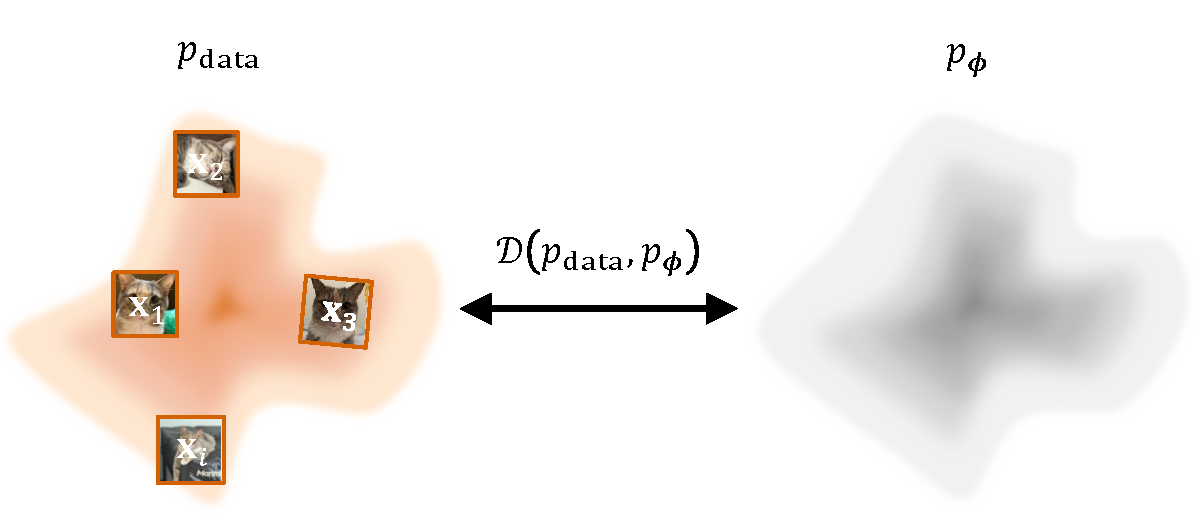
\includegraphics[width=0.9\linewidth]{Images/PartB/dgm-learning.pdf}
    \vspace{-0.2cm}
    \caption{\textbfs{DGM 中目标的图示。} 训练 DGM 本质上是最小化模型分布 $p_{\bm{\phi}}$ 和未知数据分布 $p_{\mathrm{data}}$ 之间的差异。由于 $p_{\mathrm{data}}$ 无法直接访问，因此必须使用从中提取的一组有限的独立同分布 (i.i.d.) 样本 $\rvx_i$ 来有效估计这种差异。 \figcredit{由作者创建。}}
    \label{fig:dgm-training}
\end{figure}

\paragraph{DGM 训练。}
我们学习参数 $\bm{\phi}$ 型号系列 $\{p_{\bm{\phi}}\}$ 通过最小化差异 $\mathcal{D}(p_{\mathrm{data}},p_{\bm{\phi}})$:
\begin{align}\label{eq:dgm-optimization}
  \bm{\phi}^\ast \in \arg\min_{\bm{\phi}}\; \mathcal{D}(p_{\mathrm{data}},p_{\bm{\phi}}).
\end{align}
因为 $p_{\mathrm{data}}$ 未知，实用选择 $\mathcal{D}$ 必须承认独立同分布的有效估计。\ 样本来自 $ p_{\mathrm{data}}$。有了足够的能力， $p_{\bm{\phi}^\ast}$ 可以非常近似 $p_{\mathrm{data}}$.

\subparagraph{前向 KL 和最大似然估计 (MLE)。}
我们应该如何选择模型参数以便
$p_{\bm{\phi}}$ 类似于 $p_{\mathrm{data}}$？当模型密度 $p_{\bm{\phi}}(\rvx)$ 可以评估，一个自然的想法就是让观测数据在模型下得到高密度。这导致 \emph{最大似然估计} （MLE）：我们选择
$\bm{\phi}$ 使训练样例集体分配高模型密度\footnote{对于固定观察样本 $\rvx$, 数量
$p_{\bm{\phi}}(\rvx)$，视为模型参数的函数
$\bm{\phi}$，称为 \emph{可能性}。对于连续数据，
$p_{\bm{\phi}}(\rvx)$ 是概率密度而不是准确观察的概率 $\rvx$.}。形式化这个想法的标准方法是通过（前向）Kullback-Leibler 散度\footnote{所有积分均符合勒贝格意义上的积分，并在计数度量下减少为总和。}
\begin{align*}
\mathcal{D}_{\mathrm{KL}}
\big(p_{\mathrm{data}}\|p_{\bm{\phi}}\big)
:=\;&
\int
p_{\mathrm{data}}(\rvx)
\log
\frac{p_{\mathrm{data}}(\rvx)}
     {p_{\bm{\phi}}(\rvx)}
\,\diff \rvx
\\
=\;&
\mathbb{E}_{\rvx\sim p_{\mathrm{data}}}
\big[
\log p_{\mathrm{data}}(\rvx)
-
\log p_{\bm{\phi}}(\rvx)
\big].
\end{align*}
KL 散度是不对称的，即
\[
\mathcal{D}_{\mathrm{KL}}
\big(p_{\mathrm{data}}\|p_{\bm{\phi}}\big)
\neq
\mathcal{D}_{\mathrm{KL}}
\big(p_{\bm{\phi}}\|p_{\mathrm{data}}\big).
\]

一开始，前向KL可能会出现无法使用的情况，因为数据密度
$p_{\mathrm{data}}(\rvx)$ 未知。然而，它可以分解为
\begin{align*}
\mathcal{D}_{\mathrm{KL}}
\big(p_{\mathrm{data}}\|p_{\bm{\phi}}\big)
=
\mathbb{E}_{\rvx\sim p_{\mathrm{data}}}
\left[
\log
\frac{p_{\mathrm{data}}(\rvx)}
     {p_{\bm{\phi}}(\rvx)}
\right]
=
-\mathbb{E}_{\rvx\sim p_{\mathrm{data}}}
\big[
\log p_{\bm{\phi}}(\rvx)
\big]
-
\mathcal{H}\big(p_{\mathrm{data}}\big),
\end{align*}
哪里
\[
\mathcal{H}\big(p_{\mathrm{data}}\big)
:=
-\mathbb{E}_{\rvx\sim p_{\mathrm{data}}}
\big[
\log p_{\mathrm{data}}(\rvx)
\big]
\]
是数据分布的熵。至关重要的是，这个术语不依赖于 $\bm{\phi}$。因此，虽然我们无法评价 $p_{\mathrm{data}}(\rvx)$ 本身，我们不需要知道它来优化模型参数。这给出了以下等价：
\lem{最小化 KL $\Leftrightarrow$ MLE}{mle-kl}{
\begin{align}\label{eq:MLE}
\min_{\bm{\phi}}\,
\mathcal{D}_{\mathrm{KL}}
\big(
p_{\mathrm{data}}
\,\|\,
p_{\bm{\phi}}
\big)
\;\Longleftrightarrow\;
\max_{\bm{\phi}}\,
\mathbb{E}_{\rvx\sim p_{\mathrm{data}}}
\big[
\log p_{\bm{\phi}}(\rvx)
\big].
\end{align}
}

换句话说，最小化前向KL散度相当于使真实数据样本在模型下获得高对数似然。这正是最大似然估计。在实践中，期望超过 $p_{\mathrm{data}}$ 替换为可用的训练样本
$\{\rvx^{(i)}\}_{i=1}^{N}$，假设绘制为 i.i.d.\ 来自
$p_{\mathrm{data}}$。这给出了经验负对数似然目标
\begin{align*}
\hat{\mathcal{L}}_{\mathrm{MLE}}(\bm{\phi})
:=
-\frac{1}{N}
\sum_{i=1}^{N}
\log p_{\bm{\phi}}\big(\rvx^{(i)}\big),
\end{align*}
可以使用小批量的随机梯度进行优化。因此，MLE 仅需要来自 $p_{\mathrm{data}}$;它不需要评估未知数据密度本身。 KL 散度的方向很重要，因为它决定了
\emph{差异的平均值}。对于前锋KL来说，
\[
\mathcal{D}_{\mathrm{KL}}
\big(p_{\mathrm{data}}\|p_{\bm{\phi}}\big)
=
\mathbb{E}_{\rvx\sim p_{\mathrm{data}}}
\left[
\log
\frac{p_{\mathrm{data}}(\rvx)}
     {p_{\bm{\phi}}(\rvx)}
\right],
\]
期望接管数据分布。因此，发生在以下区域 $p_{\mathrm{data}}$ 必须按型号计算。相比之下，相反的KL，
$\mathcal{D}_{\mathrm{KL}}
(p_{\bm{\phi}}\|p_{\mathrm{data}})$，对模型分布中的样本进行平均。这种差异具有重要的后果。
假设存在一个具有正数据概率的区域 $A$，
$p_{\mathrm{data}}(A)>0$，但模型在那里分配零密度，
$p_{\bm{\phi}}(\rvx)=0$ 为 $\rvx\in A$。
那么前向 KL 就变成无穷大，因为
\[
\log
\frac{p_{\mathrm{data}}(\rvx)}
     {p_{\bm{\phi}}(\rvx)}
=
+\infty
\]
在那个地区。
因此，最小化前向 KL 会严重惩罚模型的完全性能。
数据分布放置概率质量的缺失区域。
此行为通常称为 \emph{ 模式，覆盖 }。


\subparagraph{Fisher 散度.} Fisher 散度是（基于分数的）扩散建模的另一个重要概念（请参阅 \Cref{ch:score-based}）。对于两个分布 $p$ 和 $q$，定义为
\begin{align}\label{eq:fisher}
    \mathcal D_{\mathrm F}(p \|  q)
:=
\mathbb{E}_{\mathbf{x}\sim p} \left[
\left\|\nabla_{\mathbf x}\log p(\mathbf x)-\nabla_{\mathbf x}\log q(\mathbf x)\right\|_2^{2}
\right].
\end{align}
它测量 \emph{ 评分函数 } 之间的差异 
$\nabla_{\mathbf x}\log p(\mathbf x)$ 和 $\nabla_{\mathbf x}\log q(\mathbf x)$，
它们是指向更高概率区域的向量场。 
简而言之，$\mathcal D_{\mathrm F}(p \|  q)\ge 0$ 当且仅当 $p=q$ 几乎无处不在。 
它对于归一化常数是不变的，因为分数仅取决于对数密度的梯度， 
它构成了 \emph{ 分数匹配 } (\Cref{eq:ebm-sm,eq:sm}) 的基础：一种学习生成对数密度梯度的方法（基于分数的模型）。 
在此设置中，数据分布$p=p_{\mathrm{data}}$作为目标， 
而模型 $q=p_{\bm{\phi}}$ 经过训练，使其分数字段与数据的分数字段对齐。





\subparagraph{Beyond KL.} 尽管 KL 散度是最广泛使用的概率分布差异度量，但它并不是唯一的。不同的散度捕获不同的几何或统计概念的差异，这反过来又影响学习算法的优化动态。  \emph{$f$-divergences}~\citep{csiszar1963informationstheoretische} 是一个广泛的家族：
\begin{align}\label{eq:f-div}
    \mathcal{D}_f(p\|q)
=\int q(\rvx) f \left(\frac{p(\rvx)}{q(\rvx)}\right)\diff \rvx,
\qquad f(1)=0,
\end{align}
其中 $f:\mathbb{R}_+ \to\mathbb{R}$ 是凸函数。  
通过改变$f$，我们得到了许多著名的分歧：
\[
\begin{aligned}
f(u)&=u\log u &&\Rightarrow&& \mathcal{D}_f=\mathcal{D}_{\mathrm{KL}}(p\|q)\quad\text{(forward KL)},\\
f(u)&=\tfrac12 \left[u\log u-(u+1)\log \tfrac{1+u}{2}\right] &&\Rightarrow&& \mathcal{D}_f=\mathcal{D}_{\mathrm{JS}}(p\|q)\quad\text{(Jensen--Shannon)},\\
f(u)&=\tfrac12|u-1| &&\Rightarrow&& \mathcal{D}_f=\mathcal{D}_{\mathrm{TV}}(p,q)\quad\text{(total variation)}.
\end{aligned}
\]
为了清楚起见，显式形式是
\[
\mathcal{D}_{\mathrm{JS}}(p\|q)=\tfrac12 \mathcal{D}_{\mathrm{KL}}\big(p\| \tfrac12(p+q)\big)+\tfrac12 \mathcal{D}_{\mathrm{KL}}\big(q\| \tfrac12(p+q)\big),
\]
和
\[
\mathcal{D}_{\mathrm{TV}}(p,q)=\tfrac12 \int_{\mathbb{R}^D
} |p-q|\diff \rvx
=\sup_{A\subset \mathbb{R}^D } |p(A)-q(A)|.
\]
直观上，JS 散度提供了一种平滑且对称的度量，可以平衡两种分布并避免 KL 的无界惩罚（我们稍后会看到它有助于解释生成对抗网络（GAN）框架），而总变异距离捕获了两者之间最大可能的概率差异。


不同的观点来自\emph{最优传输}（参见\Cref{ch:ot-eot}），其代表是Wasserstein距离（参见\Cref{eq: Monge's Formulation}）。它衡量将概率质量从一种分布转移到另一种分布的最小成本。与比较密度比的 $f$ 散度不同，Wasserstein 距离取决于样本空间的几何形状，并且即使在 $p$ 和 $q$ 的支撑不重叠时也仍然有意义。

每个分歧都体现了分布之间不同的接近度概念，从而引发了不同的学习行为。当这些分歧在本专着的生成模型背景下自然出现时，我们将重新审视它们。







\subsection{分布建模的挑战}





























为了对复杂的数据分布进行建模，我们可以参数化概率密度函数 $p_{\mathrm{data}}$ 使用带参数的神经网络 $\bm{\phi}$，创建一个模型，我们表示为 $p_{\bm{\phi}}$。对于 $p_{\bm{\phi}}$ 要成为有效的概率密度函数，它必须满足两个基本属性：
\begin{enumerate}
    \item[(i)] \textbfs{非负性：} $p_{\bm{\phi}}(\rvx) \ge 0$ 对于所有 $\rvx$ 在域中。
    \item[(ii)] \textbfs{标准化：} 整个域上的积分必须等于 1，即 $\int p_{\bm{\phi}}(\rvx) \diff \rvx = 1$.
\end{enumerate}

网络可以自然地产生实数标量 $E_{\bphi}(\rvx) \in \R$ 用于输入 $\rvx$。为了将此输出解释为有效密度，必须对其进行转换以满足条件 (i) 和 (ii)。一个实用的替代方法是查看 $E_{\bphi}\colon\mathbb{R}^D\to\mathbb{R}$ 定义 \emph{未标准化} 密度，然后显式强制执行这些属性。


\paragraph{第 1 步：确保非消极性。}
通过对神经网络的原始输出应用正函数，我们可以保证模型的输出始终为非负值 $E_{\bm{\phi}}(\rvx)$，例如 $\abs{E_{\bm{\phi}}(\rvx)}$, $E^2_{\bm{\phi}}(\rvx)$。标准且方便的选择是指数函数。这给了我们一个非标准化的密度， $\tilde{p}_{\bm{\phi}}(\rvx)$，保证为正：
\[
\tilde{p}_{\bm{\phi}}(\rvx) = \exp(E_{\bm{\phi}}(\rvx)).
\]

\paragraph{第 2 步：强制标准化。}
功能 $\tilde{p}_{\bm{\phi}}(\rvx)$ 为正，但不积分为一。为了创建有效的概率密度，我们必须将其除以整个空间的积分。这导致了我们模型的最终形式：
\[
p_{\bm{\phi}}(\rvx) = \frac{\tilde{p}_{\bm{\phi}}(\rvx)}{\int \tilde{p}_{\bm{\phi}}(\rvx') \diff \rvx'} = \frac{\exp(E_{\bm{\phi}}(\rvx))}{\int \exp(E_{\bm{\phi}}(\rvx')) \diff \rvx'}.
\]
该表达式中的分母称为 \emph{正火常数} 或 \emph{分区函数}，表示为 $Z(\bm{\phi})$:
\[
Z(\bm{\phi}) := \int \exp(E_{\bm{\phi}}(\rvx')) \diff \rvx'.
\]
虽然此过程提供了有效的构造 $p_{\bm{\phi}}(\rvx)$，它引入了重大的计算挑战。对于大多数高维问题，计算归一化常数所需的积分 $Z(\bm{\phi})$ 很难处理。这种棘手的问题是推动许多不同系列的深度生成模型发展的核心问题。在下面的章节中，我们将介绍 DGM 的几种主要方法。每一个都旨在规避或减少评估此归一化常数的计算成本。
\newpage



\begin{figure}[th!]
\centering
\resizebox{\linewidth}{!}{
\begin{tikzpicture}[
  ->, >=Stealth, thick, font=\normalsize,
  x=2.6cm, y=2.0cm,
  every node/.style={outer sep=0pt}
]
% ============= Styles (single source of truth) =============
\tikzset{
  state/.style={
    rectangle, rounded corners=3pt,
    draw=black, fill=gray!10,
    minimum height=10mm, minimum width=14mm, % same for all variables
    align=center, inner sep=2pt,
    font=\Large % <-- enlarge text in ALL variable nodes (x, x', x_t, z, ...)
  },
  stategap/.style={ % invisible box with SAME size as state, for equal arrow lengths
    rectangle, rounded corners=3pt,
    draw=none, fill=none,
    minimum height=10mm, minimum width=14mm,
    align=center, inner sep=2pt
  },
  processor/.style={
    trapezium, trapezium stretches=true,
    trapezium left angle=80, trapezium right angle=80,
    draw=black, fill=gray!20,
    minimum height=12mm, minimum width=28mm, align=center, inner sep=2pt
  },
  ovalval/.style={
    draw, ellipse, fill=gray!10,
    minimum height=7mm, minimum width=20mm, align=center
  },
  flowblock/.style={ % NF function blocks
    rectangle, rounded corners=3pt,
    draw=black, fill=gray!20,
    minimum height=12mm, minimum width=28mm, align=center, inner sep=3pt
  }
}

% ============= Shared column anchors (perfect row alignment) =============
\coordinate (L) at (0,0);    % left column
\coordinate (M) at (2.0,0);  % (kept for reference)
\coordinate (R) at (4.8,0);  % right column
\coordinate (C) at ($ (L)!0.5!(R) $); % true midpoint between L and R

% Vertical offsets for rows
\def\rowA{0}       % Row 1: EBM
\def\rowB{-1.3}    % Row 2: AR
\def\rowC{-3.0}    % Row 3: VAE
\def\rowD{-4.7}    % Row 4: NF
\def\rowE{-7.1}    % Row 5: GAN (two floors)
\def\rowF{-8.5}    % Row 6: DM

% Row tags
\node[anchor=east] at ($(L)+(-0.5,\rowA)$) {\textbfs{EBM}};
\node[anchor=east] at ($(L)+(-0.5,\rowB)$) {\textbfs{AR}};
\node[anchor=east] at ($(L)+(-0.5,\rowC)$) {\textbfs{VAE}};
\node[anchor=east] at ($(L)+(-0.5,\rowD)$) {\textbfs{NF}};
\node[anchor=east] at ($(L)+(-0.5,\rowE)$) {\textbfs{GAN}};
\node[anchor=east] at ($(L)+(-0.5,\rowF)$) {\textbfs{DM}};

% ====================== Row 1: EBM (unchanged) ======================
\node[state]   (ebm-x)   at ($(L)+(0,\rowA)$) {$\rvx$};
\node[ovalval] (ebm-val) at ($(C)+(0,\rowA)$) {value};
\coordinate (midE) at ($ (ebm-x.east)!0.5!(ebm-val.west) $);
\node[processor, shape border rotate=270] (ebm-energy) at (midE)
  {\footnotesize\textbfs{Energy}\\[-2pt]\footnotesize $E_{\bm\phi}(\rvx)$};
\draw (ebm-x.east) -- (ebm-energy.west);
\draw (ebm-energy.east) -- (ebm-val.west);

% ====================== Row 2: AR (unchanged) =======================
\coordinate (Lb) at ($(L)+(0,\rowB)$);
\coordinate (Rb) at ($(R)+(0,\rowB)$);
\node[state]   (ar-x)    at ($ (Lb)!0/6!(Rb) $) {$\rvx_0$};
\node[state]   (ar-x0)   at ($ (Lb)!1/6!(Rb) $) {$\rvx_{1}$};
\node[state]   (ar-x1)   at ($ (Lb)!2/6!(Rb) $) {$\rvx_{2}$};
\node[state]   (ar-x2)   at ($ (Lb)!3/6!(Rb) $) {$\rvx_{3}$}; % centered at C
\node[stategap](ar-gap)  at ($ (Lb)!4/6!(Rb) $) {};
\node[state]   (ar-xLm1) at ($ (Lb)!5/6!(Rb) $) {$\rvx_{L-1}$};
\node[state]   (ar-xL)   at ($ (Lb)!6/6!(Rb) $) {$\rvx_{L}$};
\node at (ar-gap) {$\boldsymbol{\cdots}$};
\draw (ar-x.east)    -- (ar-x0.west);
\draw (ar-x0.east)   -- (ar-x1.west);
\draw (ar-x1.east)   -- (ar-x2.west);
\draw (ar-x2.east)   -- (ar-gap.west);
\draw (ar-gap.east)  -- (ar-xLm1.west);
\draw (ar-xLm1.east) -- (ar-xL.west);
% Optional arcs
\draw (ar-x.south)    to[out=-35, in=-145] (ar-x2.south);
\draw (ar-x0.south)   to[out=-40, in=-140] (ar-x2.south);
\draw (ar-gap.south)  to[out=-40, in=-140] (ar-xL.south);
\draw (ar-xLm1.south) to[out=-55, in=-125] (ar-xL.south);

% ====================== Row 3: VAE (unchanged) =======================
\node[state] (vae-x)   at ($(L)+(0,\rowC)$) {$\rvx$};
\node[state] (vae-z)   at ($(C)+(0,\rowC)$) {$\rvz$};
\node[state] (vae-xp)  at ($(R)+(0,\rowC)$) {$\rvx'$};
\coordinate (midEnc) at ($ (vae-x.east)!0.5!(vae-z.west) $);
\node[processor, shape border rotate=270] (vae-enc) at (midEnc)
  {\footnotesize\textbfs{Encoder}\\[-2pt]\footnotesize $q_{\bm\theta}(\rvz|\rvx)$};
\coordinate (midDec) at ($ (vae-z.east)!0.5!(vae-xp.west) $);
\node[processor, shape border rotate=90] (vae-dec) at (midDec)
  {\footnotesize\textbfs{Decoder}\\[-2pt]\footnotesize $p_{\bm\phi}(\rvx|\rvz)$};
\draw (vae-x.east)   -- (vae-enc.west);
\draw (vae-enc.east) -- (vae-z.west);
\draw (vae-z.east)   -- (vae-dec.west);
\draw (vae-dec.east) -- (vae-xp.west);

% ====================== Row 4: NF (unchanged) =======================
\node[state] (nf-x)  at ($(L)+(0,\rowD)$) {$\rvx$};
\node[state] (nf-z)  at ($(C)+(0,\rowD)$) {$\rvz$};
\node[state] (nf-xp) at ($(R)+(0,\rowD)$) {$\rvx'$};
\coordinate (midFwd) at ($ (nf-x.east)!0.5!(nf-z.west) $);
\coordinate (midInv) at ($ (nf-z.east)!0.5!(nf-xp.west) $);
\node[flowblock] (nf-forward) at (midFwd)
  {\footnotesize\textbfs{Forward}\\[-1pt]\footnotesize $\rvf_{\bm\phi}(\rvx)$};
\node[flowblock] (nf-inverse) at (midInv)
  {\footnotesize\textbfs{Inverse}\\[-1pt]\footnotesize $\rvf_{\bm\phi}^{-1}(\rvz)$};
\draw (nf-x.east)       -- (nf-forward.west);
\draw (nf-forward.east) -- (nf-z.west);
\draw (nf-z.east)       -- (nf-inverse.west);
\draw (nf-inverse.east) -- (nf-xp.west);

% ====================== Row 5: GAN (two floors; unchanged) =======================
\def\gansep{0.9} % vertical gap between lower and upper floors
\node[state] (gan-z)  at ($(L)+(0,\rowE)$) {$\rvz$};
\node[state] (gan-xp) at ($(C)+(0,\rowE)$) {$\rvx'$};
\coordinate (midGen) at ($ (gan-z.east)!0.5!(gan-xp.west) $);
\node[processor, shape border rotate=90] (gan-gen) at (midGen)
  {\footnotesize\textbfs{Generator}\\[-2pt]\footnotesize $\rmG_{\bm\phi}(\rvz)$};
\node[state]   (gan-x)   at ($(C)+(0,\rowE+\gansep)$) {$\rvx$};
\node[ovalval] (gan-val) at ($(R)+(0,\rowE+\gansep)$) { 0/1};
\coordinate (midDisc) at ($ (gan-x.east)!0.5!(gan-val.west) $);
\node[processor, shape border rotate=270] (gan-disc) at (midDisc)
  {\footnotesize\textbfs{Discriminator}\\[-2pt]\footnotesize $D_{\bm\zeta}$};
\draw (gan-z.east)   -- (gan-gen.west);
\draw (gan-gen.east) -- (gan-xp.west);
\draw (gan-x.east)   -- (gan-disc.west);
\draw (gan-xp.east)  -- (gan-disc);
\draw (gan-disc.east) -- (gan-val.west);

% ====================== Row 6: DM (aligned with AR; equal-length arrows) =======================
% Use the same 7 centers as AR, anchored at L and R
\coordinate (Lf) at ($(L)+(0,\rowF)$);
\coordinate (Rf) at ($(R)+(0,\rowF)$);

\node[state]    (dm-x)     at ($ (Lf)!0/6!(Rf) $) {$\rvx_0$};
\node[state]    (dm-x0)    at ($ (Lf)!1/6!(Rf) $) {$\rvx_{1}$};
\node[state]    (dm-x1)    at ($ (Lf)!2/6!(Rf) $) {$\rvx_{2}$};
\node[state]    (dm-x2)    at ($ (Lf)!3/6!(Rf) $) {$\rvx_{3}$}; % exactly the same x as AR's x_2 and C
\node[stategap] (dm-gap)   at ($ (Lf)!4/6!(Rf) $) {};
\node[state]    (dm-xLm1)  at ($ (Lf)!5/6!(Rf) $) {$\rvx_{L-1}$};
\node[state]    (dm-xL)    at ($ (Lf)!6/6!(Rf) $) {$\rvx_{L}$};

% Draw the dots on top of the invisible gap box (no effect on spacing)
\node at (dm-gap) {$\boldsymbol{\cdots}$};

% Offsets for top (dashed) and bottom (solid) channels
\def\dmshift{4.5pt}

% Forward noising (top dashed; equal visible lengths)
\draw[dashed] ([yshift=\dmshift]dm-x.east)     -- ([yshift=\dmshift]dm-x0.west);
\draw[dashed] ([yshift=\dmshift]dm-x0.east)    -- ([yshift=\dmshift]dm-x1.west);
\draw[dashed] ([yshift=\dmshift]dm-x1.east)    -- ([yshift=\dmshift]dm-x2.west);
\draw[dashed] ([yshift=\dmshift]dm-x2.east)    -- ([yshift=\dmshift]dm-gap.west);
\draw[dashed] ([yshift=\dmshift]dm-gap.east)   -- ([yshift=\dmshift]dm-xLm1.west);
\draw[dashed] ([yshift=\dmshift]dm-xLm1.east)  -- ([yshift=\dmshift]dm-xL.west);

% Reverse denoising (bottom solid; equal visible lengths)
\draw ([yshift=-\dmshift]dm-x0.west)  -- ([yshift=-\dmshift]dm-x.east);
\draw ([yshift=-\dmshift]dm-x1.west)  -- ([yshift=-\dmshift]dm-x0.east);
\draw ([yshift=-\dmshift]dm-x2.west)  -- ([yshift=-\dmshift]dm-x1.east);
\draw ([yshift=-\dmshift]dm-gap.west) -- ([yshift=-\dmshift]dm-x2.east);
\draw ([yshift=-\dmshift]dm-xLm1.west)-- ([yshift=-\dmshift]dm-gap.east);
\draw ([yshift=-\dmshift]dm-xL.west)  -- ([yshift=-\dmshift]dm-xLm1.east);

\end{tikzpicture}}
\vspace{1.0cm}
\caption{\textbfs{著名深度生成模型的计算图。} 从上到下： \textbfs{EBM} 映射输入 $\rvx$ 标量能量； \textbfs{增强现实} 生成序列 $\{\rvx_\ell\}_{\ell=0}^{L}$ 从左到右具有因果依赖性； \textbfs{VAE} 编码 $\rvx$ 到一个潜在的 $\rvz$ 并解码为重建 $\rvx'$; \textbfs{NF} 应用可逆贴图 $\rvf_\bphi$ 之间 $\rvx$ 和 $\rvz$ 和用途 $\rvf_\bphi^{-1}$ 生产 $\rvx'$; \textbfs{甘} 转换噪声 $\rvz$ 到样品 $\rvx'$ 根据真实情况判断 $\rvx$ 通过鉴别器 $D_{\bm\zeta}$; \textbfs{DM} 通过多步去噪链迭代地细化噪声样本 $\{\rvx_\ell\}_{\ell=0}^{L}$。方框表示变量，梯形是可学习网络，椭圆形是标量；箭头表示计算流程。梯形旨在表示维度变化的变换，而矩形表示保留维度的变量或映射。 \figcredit{由作者创建。}}
\label{fig:ebm-ar-vae-nf-gan-dm-unified}
\end{figure}
\newpage

\section{著名的深度生成模型}\label{sec:examples-dgm}





生成建模的一个核心挑战是学习能够捕获高维数据丰富而复杂的结构的表达性概率模型。多年来，已经开发了各种建模策略，每种策略都在易处理性、表达性和训练效率之间进行了不同的权衡。在本节中，我们将探讨一些影响该领域的最有影响力的策略，并对其计算图进行比较
\Cref{fig:ebm-ar-vae-nf-gan-dm-unified}.











\paragraph{能量模型 (EBM)。}
EBM~\citep{ackley1985learning,lecun2006tutorial} 通过能量函数定义概率分布 $ E_{\bm{\phi}}(\rvx) $ 将较低的能量分配给更有可能的数据点。数据点的概率定义为：
\begin{equation*}
    p_{\bm{\phi}}(\rvx) := \frac{1}{Z({\bm{\phi}})} \exp(-E_{\bm{\phi}}(\rvx)),
\end{equation*}
哪里 
\[Z({\bm{\phi}}) = \int \exp(-E_{\bm{\phi}}(\rvx)) \diff\rvx\] 
是配分函数。训练 EBM 通常涉及最大化数据的对数似然。然而，这需要技术来解决由配分函数的棘手性引起的计算挑战。在下一章中，我们将探讨扩散模型如何通过生成数据来提供替代方案 \emph{对数密度的梯度}，不依赖于归一化常数，从而避免了配分函数计算的需要。

















































\paragraph{自回归模型。}
深度自回归 (AR) 模型~\citep{frey1995does,larochelle2011neural,uria2016neural}
建立在一个简单但强大的观察基础上：任何联合分布都可以分解为一系列条件分布，使用 \emph{概率链式法则}。对于选定的变量顺序 $\mathbf{x}=(x_1,\ldots,x_D)$，数据分布满足
\begin{equation*}
    p_{\mathrm{data}}(\mathbf{x})
    =
    \prod_{i=1}^{D}
    p_{\mathrm{data}}(x_i | \mathbf{x}_{<i}),
    \qquad
    \mathbf{x}_{<i}=(x_1,\ldots,x_{i-1}).
\end{equation*}
重要的是，这种分解是一个精确的恒等式，而不是建模假设：任何联合分布都允许对其变量的任何选定顺序进行这种分解。挑战在于真实的条件分布
$p_{\mathrm{data}}(x_i|\mathbf{x}_{<i})$ 未知。因此 AR 模型用相同的因式分解形式参数化模型，
\begin{equation*}
    p_{\bm{\phi}}(\mathbf{x})
    =
    \prod_{i=1}^{D}
    p_{\bm{\phi}}(x_i|\mathbf{x}_{<i}),
\end{equation*}
并使用神经网络（例如 Transformer）从数据中逼近这些条件分布。例如，对于离散数据，网络可以通过 softmax 输出分类分布，而对于连续数据，它可以输出易于处理的条件密度的参数。由于每个条件分布都是标准化的，因此它们的乘积会自动定义标准化联合分布。这种结构还使得基于似然的训练变得特别简单。对于数据样本 $\mathbf{x}$，对数似然分解为
\begin{equation*}
    \log p_{\bm{\phi}}(\mathbf{x})
    =
    \sum_{i=1}^{D}
    \log p_{\bm{\phi}}(x_i|\mathbf{x}_{<i}),
\end{equation*}
因此可以直接通过最大似然或最小化负对数似然来训练模型。在训练期间，观察到的先前变量 $\mathbf{x}_{<i}$ 可用，因此通常可以并行评估其中许多条件预测。然而，生成本质上仍然是顺序的：
\begin{equation*}
    x_1 \sim p_{\bm{\phi}}(x_1),
    \qquad
    x_2 \sim p_{\bm{\phi}}(x_2| x_1),
    \qquad
    \ldots,
    \qquad
    x_D \sim p_{\bm{\phi}}(x_D|\mathbf{x}_{<D}).
\end{equation*}
因此，AR 模型提供了易于处理的精确似然性和灵活的密度建模，但采样需要一个接一个地生成变量，因此对于长序列来说，计算成本可能会很高。 AR 模型仍然是基于似然的生成模型的基础类，并且是许多现代序列和语言模型的基础。





































































































\paragraph{变分自编码器（VAE）。}
VAE~\citep{kingma2013auto} 通过引入潜变量来扩展经典自动编码器 $\rvz$ 捕获数据中的隐藏结构 $\rvx$。而不是直接学习之间的映射 $\rvx$ 和 $\rvz$，VAE 采用概率观点：他们学习 \emph{编码器}, $q_{\btheta}(\rvz|\rvx)$，它近似给定数据的潜变量的未知分布，以及 \emph{解码器}, $p_{\bphi}(\rvx|\rvz)$，它根据这些潜变量重建数据。为了使训练可行，VAE 最大化真实对数似然的易处理替代项，称为证据下界 (ELBO)：
\begin{equation*}
    \mathcal{L}_{\text{ELBO}}(\btheta, \bphi; \rvx) 
    = \mathbb{E}_{q_{\btheta}(\rvz | \rvx)} \left[ \log p_{\bphi}(\rvx | \rvz) \right] 
    - \mathcal D_{\mathrm{KL}} \left( q_{\btheta}(\rvz | \rvx) \,\|\, p_{\mathrm{prior}}(\rvz) \right).
\end{equation*}
在这里，第一项鼓励数据的准确重建，而第二项通过使潜变量接近简单的先验分布来规范它们 $p_{\mathrm{prior}}(\rvz)$ （通常是高斯分布）。  

VAE 提供了一种将神经网络与潜变量模型相结合的原则方法，并且仍然是最广泛使用的基于似然的方法之一。然而，它们也面临实际挑战，例如有限的样本清晰度和训练病态（例如解码器忽略潜变量的倾向）。尽管存在这些限制，VAE 为后来的进步（包括扩散模型）奠定了重要的基础。








\paragraph{归一化流。}
经典的基于流的生成模型包括归一化流（NF）~\citep{rezende2015variational}
以及基于神经常微分方程（NODE）的连续时间对应物~\citep{chen2018neural}，旨在学习双射映射 $\rvf_{\bm{\phi}}$ 简单潜在分布之间 $ \rvz $ 以及复杂的数据分布 $ \rvx $ 通过可逆运算符。这是通过一系列双射变换（在 NF 中）或通过将变换建模为常微分方程（在 NODE 中）来实现的。这些模型利用“密度变量替换公式”，支持 MLE 训练：
\begin{equation*}
    \log p_{\bm{\phi}}(\rvx) = \log p(\rvz) + \log \left| \det \frac{\partial \rvf_{\bm{\phi}}^{-1}(\rvx)}{\partial \rvx} \right|,
\end{equation*}
哪里 $ \rvf_{\bm{\phi}} $ 表示可逆变换映射 $ \rvz $ 至 $ \rvx $。 NF 使用可逆变换和易于处理的雅可比行列式显式地对归一化密度进行建模。通过变量替换公式分析吸收归一化常数，使似然计算精确且易于处理。尽管概念上很优雅，但经典的基于流的模型常常面临实际限制。例如，NF 通常会施加限制性的架构约束以确保双射性，而 NODE 可能会因求解 ODE 的计算开销而遇到训练效率低下的问题。这两种方法在扩展到高维数据时都面临挑战。在后面的章节中，我们将探讨扩散模型如何与这些经典的基于流的方法相关并建立在这些方法的基础上。




















































\paragraph{生成对抗网络（GAN）。}
GAN~\citep{goodfellow2014generative} 由两个神经网络、一个生成器组成 $ \rmG_{\bm{\phi}} $ 和鉴别器 $ D_{\bm{\zeta}} $，相互竞争。生成器旨在创建真实的样本 $ \rmG_{\bm{\phi}}(\rvz) $ 来自随机噪声 $ \rvz \sim p_{\mathrm{prior}}$，而鉴别器尝试区分真实样本 $ \rvx $ 并生成样本 $ \rmG_{\bm{\phi}}(\rvz) $。 GAN 的目标函数可以表示为：
\begin{equation*}
    \min_{\rmG_{\bm{\phi}}} \max_{D_{\bm{\zeta}}} \underbrace{\mathbb{E}_{\rvx \sim p_{\mathrm{data}}(\rvx)}[\log D_{\bm{\zeta}}(\rvx)]}_{\text{real}} + \underbrace{\mathbb{E}_{\rvz \sim p_{\mathrm{prior}}(\rvz)}\left[\log(1 - D_{\bm{\zeta}}\left(\rmG_{\bm{\phi}}(\rvz))\right)\right]}_{\text{fake}}.
\end{equation*}
GAN 没有定义明确的密度函数，因此完全绕过似然估计。他们不是计算归一化常数，而是专注于生成密切模仿数据分布的样本。 

从散度的角度来看，判别器隐式地测量真实数据分布之间的差异 $p_{\mathrm{data}}$ 
和发电机分布 $p_{\rmG_{\bphi}}$，其中 $p_{\rmG_{\bphi}}$ 表示生成样本的分布 $\rmG_{\bphi}(\rvz)$ 从噪声中获得 $\rvz \sim p_{\mathrm{prior}}$。使用固定生成器的最佳判别器 $\rmG_{\bphi}$ 计算为
\begin{equation*}
     \frac{p_{\mathrm{data}}(\rvx)}{p_{\mathrm{data}}(\rvx) + p_{\rmG_{\bphi}}(\rvx)},
\end{equation*}
发电机的最小化减少到
\begin{equation*}
    \min_{\rmG_{\bphi}} \; 2\,\mathcal{D}_\mathrm{JS} \left(p_{\mathrm{data}} \,\|\, p_{\rmG_\bphi}\right) - \log 4.
\end{equation*}
在这里， $\mathcal{D}_\mathrm{JS}$ 表示 Jensen-Shannon 散度，定义为
\begin{equation*}
    \mathcal{D}_\mathrm{JS}(p \,\|\, q) 
    := \tfrac{1}{2} \mathcal{D}_\mathrm{KL} \left(p \,\middle\|\, \tfrac{p+q}{2}\right) 
    + \tfrac{1}{2} \mathcal{D}_\mathrm{KL} \left(q \,\middle\|\, \tfrac{p+q}{2}\right).
\end{equation*}
这表明 GAN 隐式最小化 $\mathcal{D}_\mathrm{JS}(p_{\mathrm{data}} \,\|\, p_{\rmG_\bphi})$。更广泛地说，扩展例如 $f$-GAN~\citep{nowozin2016f} 通过证明对抗性训练可以最小化一个家庭来概括这一观点 $f$-分歧，将 GAN 置于与其他生成模型相同的分歧最小化框架内。尽管 GAN 能够生成高质量的数据，但其最小-最大训练过程非常不稳定，通常需要精心设计的架构和工程技术才能获得令人满意的性能。然而，GAN 已作为辅助组件复活，以增强其他生成模型，特别是扩散模型。






\newpage
\section{建模分类}\label{sec:taxonomy}



正如我们所见，DGM 涵盖了广泛的建模策略。一个根本的区别在于这些模型如何 \emph{参数化} 底层数据分布，即是否指定 $p_\bphi(\mathbf{x})$ \emph{明确} 或仅 \emph{隐式}，无论训练目标如何。

\begin{itemize}
  \item \textbfs{显式模型：}  
  这些模型直接参数化概率分布 $p_\bphi(\mathbf{x})$ 通过易处理或近似易处理的密度或质量函数。示例包括 AR、NF、VAE 和 DM，所有这些都定义 $p_\bphi(\mathbf{x})$ 精确地或通过易于处理的边界。

  \item \textbfs{隐式模型：}  
  这些模型仅通过采样过程指定分布，通常采用以下形式 $\mathbf{x} = \rmG_\bphi(\mathbf{z})$ 对于某些噪声变量 $\mathbf{z} \sim p_{\mathrm{prior}}$。在这种情况下， $p_\bphi(\mathbf{x})$ 不以封闭形式提供，并且可能根本没有定义。
\end{itemize}


表中 \Cref{tb:comparison-explicit-implicit} 提供了这些对比方法的简洁总结。
\begin{table}[th]
  \caption{显式和隐式生成模型的比较}
  \small
  \centering
  \resizebox{\textwidth}{!}{
  \begin{tabular}{cccc}
    \toprule
    & \multicolumn{2}{c}{\textbfs{显式}} & \textbfs{隐式} \\
    \cmidrule(lr){2-3}
    & \textbfs{精确似然} & \textbfs{近似\ 似然} & \\
    \midrule
    \textbfs{可能性}
      & 易处理
      & 绑定/大约。
      & \makecell{非直接建模/\\难处理} \\

    \textbfs{目标}
      & MLE
      & ELBO
      & 对抗性 \\

    \textbfs{示例}
      & NF、AR
      & VAE、DM
      & GAN \\
    \bottomrule
  \end{tabular}
  }
  \label{tb:comparison-explicit-implicit}
\end{table}


\paragraph{连接至扩散模型。}
总而言之，这些经典的 DGM 系列说明了复杂分布建模的互补策略。  
除了其独立的重要性之外，它们还提供了理解扩散模型的指导原则。  
扩散方法继承了其中几个观点的思想：它们通过变分训练目标连接到 VAE，通过学习对数密度梯度（与能量函数密切相关）的分数匹配方法连接到 EBM，并通过连续时间变换连接到 NF。  

为了为后面章节中讨论的扩散方法奠定基础，我们将重点关注三个中心范式：VAE (\Cref{sec:vae})、EBM (\Cref{sec:ebm}) 和 NF (\Cref{sec:flow-based-method})。  
这种探索为现代基于扩散的生成模型的核心原则奠定了基础，这些原则将在接下来的章节中进一步发展。











\newpage
\section{结束语}\label{sec:ch1_cr}


本章建立了深度生成建模的基本概念。我们首先定义主要目标：学习一个易于处理的模型分布 $p_{\text{model}}$（由 $\bm{\phi}$ 参数化），它近似于未知的复杂数据分布 $p_{\text{data}}$。一个主要挑战是归一化常数或配分函数 $Z(\bm{\phi})$ 的计算困难性，这是定义有效概率密度所必需的。



为了解决这个问题，人们开发了各种深度生成模型，每个模型都采用了不同的策略。我们调查了几种著名的方法，包括能量模型（EBM）、自回归模型（AR）、变分自编码器（VAE）、归一化流（NF）和生成对抗网络（GAN）。这些模型可以大致分为显式模型和隐式模型，显式模型定义易于处理的密度，隐式模型仅通过采样过程定义分布。虽然这些经典框架中的每一个都很重要，但其中三个尤其是作为本专着重点关注的扩散模型的概念起源：VAE、EBM 和 NF。在接下来的章节中，我们将从这三个基本范式追溯扩散模型的演变：
\begin{enumerate}
    \item B 部分将从探索变分视角 (\Cref{ch:variational}) 开始，展示 VAE（的分层潜变量结构）如何自然地导致去噪扩散概率模型 (DDPM) 的制定。
    \item 接下来，我们将研究基于分数的视角（\Cref{ch:score-based}），它起源于 EBM 和分数匹配，并发展为噪声条件分数网络（NCSN）和更通用的分数 SDE 框架（\Cref{ch:score-sde}）。
    \item 最后，我们将研究基于流的视角（\Cref{ch:flow-based}），它建立在将流规范化到帧生成作为连续转换的原则之上，并通过流匹配的概念进行概括。
\end{enumerate}

通过了解这些起源，我们将建立一个连贯的框架来解释扩散模型的不同表述并揭示统一它们的深层原理。